\documentclass[12pt, french]{article}

\usepackage{fancyhdr, fancybox, lastpage, wrapfig}
\usepackage[most]{tcolorbox}
\usepackage[a4paper, margin={0.3in, .75in}]{geometry}
\usepackage[utf8]{inputenc}

\pagestyle{fancy}
\renewcommand\headrulewidth{1pt}
\renewcommand\footrulewidth{1pt}
\fancyhf{}
\rhead{ \em{Zakaria Haouzan}}
\lhead[C]{\em{1ére année baccalauréat Sciences Mathématiques}}
\chead[C]{}
\rfoot[C]{}
\lfoot[R]{}
\cfoot[]{\em{Page \thepage / \pageref{LastPage}}}


\newtcolorbox{Box2}[2][]{
                lower separated=false,
                colback=white,
colframe=white!20!black,fonttitle=\bfseries,
colbacktitle=white!30!gray,
coltitle=black,
enhanced,
attach boxed title to top left={yshift=-0.1in,xshift=0.15in},
title=#2,#1}


\begin{document}
\begin{center}
   \shadowbox {\bf{Suivi d’une Transformation Chimique}}
\end{center}


%%_________________________Exercice ! :"_________________________Exercice
   \begin{Box2}{Exercice 1 : }
La combustion complète dans le dioxygène de l’air de l’éthanol de formule $C_2H_6O$ produit du dioxyde de
carbone et de l’eau.
\\1. Écrire l’équation bilan de la réaction de combustion
\\2. On fait brûler une masse de $6,8$ g d’éthanol dans le dioxygène de l’air
\\ 2.a. Établir le tableau d'avancement (le dioxygène est un réactif en excès)
\\ 2.b. Calculer les masses d’eau et de dioxyde de carbone obtenues
\\ 2.c. Calculer dans les CNTP le volume de dioxygène nécessaire à la combustion
   \end{Box2}


%%_________________________Exercice !2 :"_________________________Exercice
\begin{Box2}{Exercice 2 : }
   Une solution aqueuse d’acide chlorhydrique $H^+_{(aq)} + Cl^{-}_{(aq)}$ réagit avec le magnésium solide $Mg(s)$ . on obtient un dégagement de dihydrogène et il se forme des ions magnésium $Mg^{2+}_{(aq)}$.
   \begin{enumerate}
   \item  Écrire l’équation de la réaction
   \item On introduit dans un flacon une masse m = 27g de magnésium et on ajoute 40ml de solution d’acide chlorhydrique de concentration molaire C = 1, 0 mol/l , on bouche rapidement le flacon et en utilisant un manomètre digitale, on mesure la pression finale dans le flacon .
      \begin{enumerate}
         \item Déterminer les quantités initiale des réactifs .
         \item À l’aide d’un tableau d’avancement , déterminer l’avancement final et le réactif limitant .
      \end{enumerate}
\item Lorsque le dégagement gazeux cesse , déterminer :
   \\(a) La quantité de dihydrogène formé
   \\(b) La pression de d’hydrogène dans les conditions de l’expérience où le volume occupé
par les gaz vaut $1, 1L$ et la température est de 20◦C .
   \\(c) La pression finale qui sera affichée par le manomètre si la pression initiale est égale à $1020hPa$
\\Données : M(Mg) = 24g/mol , M(H) = 1g/mol
\end{enumerate}
\end{Box2}

%%_________________________Exercice ! 3:"_________________________Exercice
\begin{Box2}{Exercice 3 :}
  
   \begin{wrapfigure}[12]{r}{0.3\textwidth}
  \begin{center}
    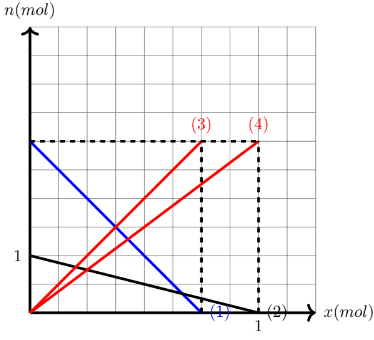
\includegraphics[width=0.3\textwidth]{./img/img00.png}
  \end{center}
\end{wrapfigure}

   Le graphe de coté représente l’évolution, en fonction de l’avancement de la réaction x, des quantités de matière des réactifs et des produits  d’une réaction se produisant dans le haut fourneau. Les réactifs sont la magnétite $Fe_3O_4$, le monoxyde de carbone CO, les produits sont le fer et le dioxyde de carbone.

1. Écrire l’équation de cette réaction en utilisant les nombres stœchiométriques entiers les plus petits possibles .

2. Comparer le nombre stœchiomètrique de chaque espèce et le coefficient directeur de la droite correspondante.

3. A partir du graphe déterminer : l’avancement maximal de la réaction et le réactif limitant la composition (mol) de l’état initial et de l’état final.

courbe(1):CO , courbe(2):magnétite ,courbe(3):CO2 ,courbe(4): Fe.
\end{Box2}

\vspace{2cm}
\begin{center}
   \Large{ \em{Exercices Supplémentaires}}
\end{center}


%%_________________________Exercice 4 : _________________________Exercice
\begin{Box2}{Exercice 4 : }
  \begin{wrapfigure}[12]{r}{0.3\textwidth}
  \begin{center}
    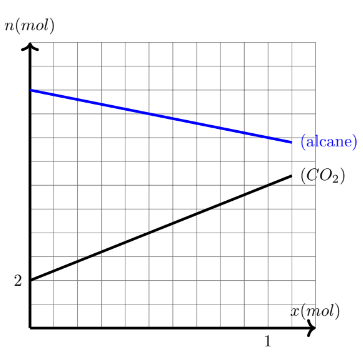
\includegraphics[width=0.3\textwidth]{./img/img01.png}
  \end{center}
\end{wrapfigure}


Les alcanes sont des hydrocarbure de formule brute $C_nH_{2n+2}$ . Pour déterminre la formule brute d’un alcane, on réalise sa combustion complète .

1. Écrire l’équation de la réaction de combustion complète d’un alcane dans le dioxygène avec le nombre stœchiométriques 1 pour l’alcane .

2. Les graphes de coté représentent l’évolution des quantités de matière de l’alcane et du dioxyde de carbone en fonction de l’avancement x de la réaction .

a. À l’aide des graphes , déterminer la composition , en quantité de matière , du système dans l’état initiale sachant que $n_i(O_2) = 7, 0 mol$ et $n_i(H_2O) = 0 mol$ .

b. En utilisant un tableau d’avancement et les graphes , calculer la valeur de n et en déduire la formule brute de l’alcane . 

c. Déterminer l’avancement final, le réactif limitant et la composition en quantité de matière , du système dans l’état final .
\end{Box2}


%%_________________________Exercice 5 : _________________________Exercice
\begin{Box2}{Exercice 5 : }
Un composé organique gazeux A, a pour formule $ C_xH_y$ où $x$ et $y$ sont des nombres entiers.

   1. On réalise la combustion complète d’une masse m=1g de composé A en présence d’un excès de dioxygène. La réaction produit m1=1,64g d’eau. Écrire l’équation-bilan de la réaction de combustion.

   2. L’échantillon A de masse 1g occupe un volume V=545 mL dans les conditions de l’expérience où le volume molaire est Vm = 24 L.mol-1 . Quelle est la masse molaire du compose A ? On suppose que le gaz se comporte comme un gaz parfait.

   3. Déduire des résultats des questions précédentes la formule brute du compose A.

   4. Quel volume minimal de dioxygène faut-il mettre en œuvre pour réaliser la combustion complète de 15 kg du compose A ?
\end{Box2}

%%_________________________Exercice 6 : _________________________Exercice

\begin{Box2}{Exercice 6 :}
La combustion complète dans le dioxygène de $224 cm^3$ d'un corps pur gazeux de formule $C_nH_{2n+2}$ a donné $896 cm^3$ de dioxyde de carbone et de l'eau.

   1. Ecrire l'équation bilan de la réaction et déterminer la formule de ce corps pur

   2. La combustion dans le dioxygène de 1L d'un hydrocarbure gazeux $C_xH_y$ a nécessité 5L de dioxygène et a donné 3L de dioxyde de carbone. Ecrire l'équation bilan de la réaction et déterminer la formule brute de l'hydrocarbure

   \textbf{NB : Les volumes sont mesurés dans les mêmes conditions}
\end{Box2}


%%_________________________Exercice 7 : _________________________Exercice


%%_________________________Exercice 8 : _________________________Exercice


\end{document}
